\section{Results}
Our study aims to exhibit and characterize the fine-grained search patterns of the human mind, when confronted with a hard problem. Here, the hard problem consists in being incentivized to reverse-engineering a Bayesian network (a standard task to probe {\bf XXXX} in cognitive science \cite{}) with 3-nodes (treatmend 1 : 8 conditional probabilities) and with 4 nodes (treatment 2: 16 conditional probabilities). Our fine-grained capture of trials (at 1 second resolution over 40 minutes) allows us to characterize the fine-grained dynamics of human search in abstract spaces. At first sight, the patterns resemble those of resource hunting by animals \cite{}�and humans hunter-gatherers \cite{}, yet with some specificities, which seem to limit human performance when solving abstract problems.\\

In this section, we first characterize the anomalous super-diffuse nature of the search process, and explain how it differs from other animal and human search patterns found. We then turn to define and characterize how much individuals tend to explore beyond their ``cognitive frontier" versus trying to re-arrange from within the space they have explored already. We finally show memory plays a special role in the search process, and we exhibit some trade-offs that humans seem to face when they attempt to converge to the correct Bayesian network design.

%\begin{figure}[h!]
%\begin{center}
%\includegraphics[width=12cm]{figures/figure2.eps}
%\caption{\footnotesize{Simplified diagram of exploration and recombination on a plane: {\bf A. Recombination:} iteration {\bf e'} does not incorporate new information. It is a convex combination of all previous proposed solutions (i.e., $\{a,b,c,d\}$).  {\bf B. Exploration:} the average distance between iteration {\bf e} and all previous iterations is larger than half of the maximum distance between any previous proposed solutions. Exploration is not memoryless: {\bf e} is closer to {\bf c} and {\bf d} than {\bf a} and {\bf b}. }}
%\label{fig:2}
%\end{center}
%\end{figure}

\subsection{An anomalous Super-Diffusive Process}
Humans, like many other animals \cite{viswanathan1996levy,ramos2004levy,reynolds2007displaced}, use efficient strategies to search for resources over large areas \cite{brown2007levy,rhodes2007human}. These L\'evy walk strategies alternate between many small local displacements and a few long range displacements. Namely, the distribution of displacements obeys a power law: 

\begin{equation}
\label{displacements}
pdf(\Delta r) = \Delta r^{-\alpha -1}.
\end{equation}

We find that displacements between proposed models (on average over all participants) follow a similar power law distribution with $\alpha = 0.40(5)$ (see Figure \ref{fig:1}B). In addition, the distribution of waiting times $\Delta t$ between two iterations of model propositions, also follows a power law: 

\begin{equation}
\label{wtimes}
pdf(\Delta t) = \Delta t^{-\beta -1},
\end{equation}

with 2 regimes : $\beta_{\Delta t < 125} = 0.38(4)$ and $\beta_{\Delta t > 125} = 1.59(5)$. Distributions of $\Delta r$ and $\Delta t$ are equivalent for the simple and complex treatments. Together, equations \ref{displacements} and \ref{wtimes} define a Continuous Time Random Walk (CTRW) \cite{montroll1965random}, a process which describes another flavour of foraging search in ecological systems \cite{book_ecological_systems,humphries2014optimal}. The observed displacement exponent is significantly smaller, compared to optimal L\'evy walks of search in ecosystems, typically found close to  $\alpha = 1$ \cite{reynolds2007displaced}. Such an exponent is mathematically optimal for search of sparse solutions in large problem spaces, where it is naively assumed that search is a memoryless process \cite{viswanathan1999optimizing, edwards2007revisiting,song2010modelling,viswanathan2011physics}. \\

\subsection{Memory in L\'evy Walks/Flights}

Unlike such naive memoryless processes, human search exhibits repetition, which implies that humans make use of their memory on all time scales. For instance, evidence from online auctions \cite{radicchi2012rationality}  suggests that an optimal search strategy ($\alpha = 2 $) can be reached by humans when they are subjected to evolutionary forces \cite{radicchi2012evolution}. 
Sedentary humans (e.g., living in cities) also exhibit repeated mobility patterns, such as travel between home and work places, with short displacements around a few areas of particular interest.  These regularities are punctuated by travels beyond the borders of the city, to other cities, regions or countries \cite{brockmann2006scaling,gonzalez2008understanding,song2010modelling}. 
Using mobile phone traces, Song et al.  have proposed a modified version of L\'evy flights, by incorporating a form of preferential attachment, which predicts that most visited places tend to get even more visits \footnote{The model proposed by Song et al. \cite{song2010modelling} is however a challenge to common sense logic: Most visited places (i.e., home and workplace) are visited at a stable rate, roughly following circadian periods.}. Yet, on the contrary to early models \cite{viswanathan1999optimizing, edwards2007revisiting,song2010modelling,viswanathan2011physics}, proposed explanations by Radicchi et al. \cite{radicchi2012evolution} and Song et al. \cite{song2010modelling} incorporate memory, either through evolutionary forces to optimise online auction strategies (the best strategies survive), or human memory driving routine repeated visits of the same places \cite{gonzalez2008understanding,song2010modelling}, simply because they are remembered to bring resources--financial resources are derived from staying at work, while being at home allows for rest and the rewards of home life).\



\subsection{L\'evy Flight / CTRW}
We first find that the search process approximately follows a continuous time L\'evy flight process, where waiting times between moves are random variables.  Both the distributions of displacement (Figure \ref{fig:pdfs}A ) and waiting times (Figure \ref{fig:pdfs}B ) are best described by power law distributions  (Probability density function of displacement $pdf(\Delta r) = \Delta r^{-\alpha -1}$ with $\alpha = 0.40(5)$.  Note that this is NOT a L\'evy flight (for which $\alpha$ would have to be between 1 and 3.  {\bf B.} Probability density function of waiting time $\Delta t$ $pdf(\Delta t) = \Delta t^{-\beta -1}$ with 2 regimes : $\beta_{\Delta t < 125} = 0.38(4)$ and $\beta_{\Delta t > 125} = 1.59(5)$. Distributions of $\Delta r$ and $\Delta t$ are equivalent for the simple and complex treatments.)

{\bf Problem :} Such CTRW process are generally expected to follow ballistic diffusion characterized by mean square displacement (MSD) and diffusion $\sim t^{\mu}$ with  $\mu_{Levy} = 1$ \
or super-diffusion $\mu_{CTRW} = \beta$ \cite{21,23}). Here, however, mean square displacement (MSD) decays as $\sim t^{\mu}$ with $\mu_{simple} =-0.23(2)$ and $\mu_{complex} =-\
 0.26(1)$ showing a much slower convergence than is generally expected.



\begin{figure}[h!]
\begin{center}
\includegraphics[width=17cm]{figures/figure1.eps}
\caption{\footnotesize{{\bf A.} Average Jensen-Shannon Distance $\langle D \rangle$ decays as a function of time as $\sim t^{\nu}$ with $ \nu \approx -0.15(1)$ indicating a very slow convergence to the true model {\bf [indicate $t_0$s and what their values may mean]}. {\bf B.} Probability density function of displacement $pdf(\Delta r) = \Delta r^{-\alpha -1}$ with $\alpha = 0.40(5)$ with a cut-off limited by the largest possible displacement, which is $\sqrt{k}$ with $k$ the number of conditional probabilities to evaluate. {\bf C.}  Probability density function of waiting time $\Delta t$ $pdf(\Delta t) = \Delta t^{-\beta -1}$ with 2 regimes : $\beta_{\Delta t < 125} = 0.38(4)$ and $\beta_{\Delta t > 125} = 1.59(5)$. Distributions of $\Delta r$ and $\Delta t$ are equivalent for the simple and complex treatments.}}
\label{fig:1}
\end{center}
\end{figure}




\begin{figure}[h!]
\begin{center}
\includegraphics[width=16cm]{figures/Dmin_vs_St.eps}
\caption{{\bf A.} Minimum Euclidian distance $D_{min}$ (between the best model and the true model) exhibits a scaling as a function of the number of distinct sites visited $S_{T}$. $D_{min} \sim S_{T}^{\gamma}$ with resp. $\gamma_{simple} = -0.20(4)$ and $\gamma_{complex} = - 0.13(3)$. {\bf B.}  The number of visited sites over time $S_t$ is a linear function of time $t$. Hence, the number of distinct visited sites is a predictor of the minimum distance $D_{min}$ achieved. The result also holds for average distance. {\bf C.}  Mean square displacement (MSD) decays as $\sim t^{\mu}$ with $\mu_{simple} =-0.23(2)$ and $\mu_{complex} =- 0.26(1)$ showing a slow convergence (on the contrary of a normal L\'evy flight / CTRW, which is characterized by respectively diffusion $\mu_{Levy} = 1$ or super-diffusion $\mu_{CTRW} = \beta$ \cite{21,23}). All colored areas show the 25th percentile confidence intervals.}
\label{fig:Dmin_vs_St}
\end{center}
\end{figure}


\subsection{Explore versus Exploit}


\begin{figure}[h!]
\begin{center}
\includegraphics[width=18cm]{figures/EE.eps}
\caption{{\bf A.} Explore / Exploit ($EE$ )as a function of displacement $\Delta r$. {\bf B.} $\Delta D_{jsd}$ as a function Explore / Exploit: Improvement seems better for $EE \approx 1.4$. {\bf C.} $D_{jsd}$ as a function of $EE$: As distance gets smaller, a balance around $EE = 1$ seems to be reached.}
\label{fig:pdf_return}
\end{center}
\end{figure}


\subsection{Memory, Return to previously visited sites \& Recombination}
For both experimental treatments of the Bayesian network reverse engineering experiment \cite{castnerForthcoming}, participants made use of various time scales of memory as they returned to previous model iterations, following a power law (see Figure \ref{fig:2}A and SI \ref{solutionspace_partitions} for details on solution space partitioning).\\

%\begin{figure}[h!]
%\begin{center}
%%\includegraphics[width=16cm]{figures/Figure1.eps}
%\caption{\footnotesize{{\bf A.} return to previously visited sites : $\mathrm{pdf}(V_r) \sim {V_r}^{- \gamma -1}$, with $\gamma_{simple} = 1.6(1)$ and $\gamma_{complex} = 1.5(1)$ $\rightarrow$ tendency to return to previously visited sites : This goes against the imperative to visit new sites (maximize $S_T$) in order to reduce $D_{min}$ (c.f. Figures \ref{fig:Dmin_vs_St}B and \ref{fig:Dmin_vs_St}C). Moreover, given the size of the parameter space [the simplex of dimension $10^{8}$ (resp. $10^{16}$) in the simple (resp. complex) case], it is remarkable that participants tend to return to exactly the same infinitesimal spots in this space. This suggest memory dependent stickiness. {\bf B.} Influence of a model proposed at some time, $t$ in subsequent models at some $t +s$, with $s \geq 1$. The influence is computed as 1/distance between the focal model and subsequent models. On average over all participants in each treatment, influence $I$ decays as $I \sim t^{-\chi}$ with $\chi = 0.48(2)$ ($p < 0.01$ and $R > 0.32$). This result shows that the importance of a memory decays slowly, with implications for the convergence of beliefs to the processes that are the content of those beliefs.}}
%\label{fig:3}
%\end{center}
%\end{figure}

\begin{figure}[h!]
\begin{center}
\includegraphics[width=10cm]{figures/schematic_displacement.eps}
\caption{2-dimensional schematic description of the {\it L\'evy flying mind} model ({\bf ``Proportional Attraction"}): At each time step, the individual must choose between remaining in the solution envelope that has already been explored and exploring outside the currently known solution envelope.  We assign some probability $p$ (a number between 0 and 1) to the participant's decision of staying in the explored envelop and probability $1-p$ to the decision to explore outside that envelop.  If it is harder to find solutions that offer a balanced re-combination of previous solutions than to think out-of-the-box and propose solutions outside of the current solution envelope, then $p < \frac{1}{2}$ else $p \geq \frac{1}{2}$.}
\label{fig:schematic}
\end{center}
\end{figure}




``cognitive load"

{\bf [waiting times? ]}

Memory plays a central role in recombining multiple previously explored models into new ones. We find strong influence of a focal model on subsequent models. On average over all participants in each treatment, influence $I$ decays as $I \sim t^{-\chi}$ with $\chi = 0.48(2)$ ($p < 0.01$ and $R > 0.32$)  (Figure \ref{fig:2}B). Because the time decay exhibits a power law with exponent $\chi < 1$, on average, models proposed in the past never vanish from memory, and may be reused or inspire future models. If we assume that the rate of proposed models remains roughly constant  over time for some participant, as time passes it gets statistically harder to come up with novel solutions ``because mental constructions are imprinted by past experience'' and the cognitively low hanging fruits as well as all of their combinations are being used up, leaving less and less intuitive solutions in the unexplored space of models. Often--as in the Monty Hall example--the true processes of stochastic influence and their observational consequences are highly counter-intuitive.  


\begin{figure}[h!]
\begin{center}
\includegraphics[width=15cm]{figures/memory.eps}
\caption{{\bf A.} Influence of a model proposed at time in subsequent models. The influence is computed as 1/distance between the focal model and subsequent models. On average over all participants in each treatment, influence $I$ decays as $I \sim t^{-\chi}$ with $\chi = 0.48(2)$ ($p < 0.01$ and $R > 0.32$). This result shows that memory is a long memory process, with implications for the convergence to. {\bf B.} Return to previously visited sites : $\mathrm{pdf}(V_r) \sim {V_r}^{- \gamma -1}$, with $\gamma_{simple} = 1.6(1)$ and $\gamma_{complex} = 1.5(1)$ $\rightarrow$ tendency to return to previously visited sites : This goes against the imperative to visit new sites (maximize $S_T$) in order to reduce $D_{min}$ (c.f. Figures \ref{fig:Dmin_vs_St}B and \ref{fig:Dmin_vs_St}C). Moreover, given the large number of sites [$10^{8}$ (resp. $10^{16}$) in the simple (resp. complex) case], it is remarkable that participants tend to return to exactly the same (tiny) spots. This suggest some stickiness of memory. {\bf C.}  Schematic representation of remix dynamics. The color bars show the proportion (i.e., $1/d$) of previously proposed solutions in solution proposed at time $t$. New colors are introduced 	tosignal exploration. From time to time, individuals return to previously visited solutions (signaled by $r$).}
\label{fig:pdf_return}
\end{center}
\end{figure}

\subsubsection{Implications of Memory and Exploration on Performance}
Individuals deploy {\it exploration}, {\it exploitation}, and {\it return} strategies in order to get closer to the best solutions (i.e., factorizations of the joint distribution that are indistinguishable from the true model). Each move may lead to improvement (i.e., reduction of cognitive distance to the true model) or, on the contrary, to dis-improvement. 

We find that displacement has an influence on improvement. As one could surmise, small displacements can only bring marginal improvement, while larger displacements bring more opportunities for improvement, yet at the cost of potential short-term losses that may be quite large. Large displacements ($\Delta r > 0.2$) can bring rather negative performance. Figure \ref{fig:vs_dr} shows the evolution of the distance to the true model $D$ as a function of displacement $\Delta r$. The distance scales as $D \sim {\Delta r}^{\mu}$ with $\mu_{simple} = 0.88(1)$ [resp. $\mu_{complex} = 082(2)$]. For $\Delta r > 0.2$, $D$ uncertainty quickly balloons, but rather positive, reflecting the {\it cost} of making ``wild'' innovations. 

There is no clear relation between time spent on taking the decision to move and performance {\bf [show $\Delta D_{jsd}$ versus $\Delta t$] if relevant: question here is the functional form of how time spent on cognitive processing leads to better or worse results.}.

While there is no clear relation between time spent between moves and performance {\bf [$\Delta D_{jsd}$ versus $\Delta t$]}, the decision to make a larger displacement takes more time. For $\Delta r < 0.2$, the processing time before a displacement decision is made scales as $\Delta t \sim \Delta r^{\gamma}$ with $\gamma_{simple} = 0.11(1)$ [resp. $\gamma_{complex} = 0.13(1)$]. For $\Delta r > 0.2$, the processing times before a displacement decision is taken get disproportionally long (up to tens of seconds on average for a displacement of 0.7 (i.e., $\approx 25\%$ of the maximum displacement distance). On both panels, blue and red areas show the $25^{th}$ percentile confidence intervals.


The minimum distance $D_{min}$ (between the best model and the true model) exhibits a scaling as a function of the number of distinct sites visited $S_{T}$. $D_{min} \sim S_{T}^{\gamma}$ with resp. $\gamma_{simple} = -0.20(4)$ and $\gamma_{complex} = - 0.13(3)$. {\bf C.} The logarithm of number of visited sites is a linear function of the logarithm of time $t$. Hence, the number of distinct visited sites is a predictor of the minimum distance $D_{min}$ achieved at time $t$. The result also holds for groupings with averaged cognitive distances.


\subsubsection{Recombination of previously proposed solutions}

{\bf Depending on the questions at stake, one must factor human timing either as delayed reactions to externally timed external events, or as part of cognitive processing, or both. We hold the timing of observed events constant in an experimental setting and we are interested in the processes of the mind.}

Recombination of past proposed models accounts for XX\% of moves, and yields on average  YY\% performance. It is a fine-tuning optimization search within the already explored solution envelop.


\subsubsection{Exploration of solutions beyond the convex hull}
We are interested in proposed models, which go beyond the solution space (convex hull) known at iteration $i$. If twice $\langle D_{jsd,i} \rangle$, the average distance of solution $j$ compared to all previous solutions $i < j$, is larger than $ max(D_{jsd})$ the maximum distance between 2 solutions in $iterations = \{1,...,i\}$, then the new proposed model {\it {\bf incorporates causal hypotheses and conditional independence assumptions, which are not entailed by previously explored models}} and contributes to the enlargement of the currently explored joint-hypotheses space. To measure how much a proposed model is explorative, versus exploitative of causal and conditional independence structures, we define the ratio:

\begin{equation}
EE_{j} = \frac{2 \langle D_{jsd,j} \rangle}{max(D_{jsd,1,...,j})}.
\end{equation}

For $EE < 1$, the individual is choosing an exploitative solution, that lies within the boundaries of the convex hull of already explored solutions. For $EE \approx 1$, the proposed solution is on -- or close to -- the boundaries, and for $EE > 1$, the proposed solution is outside the convex hull, and therefore explorative. The larger $EE$, the more explorative the proposed solution. For both 3-node and 4-node BN treatments,  the number of explorative moves is over all people much larger than exploitative ones :  $5416$ vs. $1873$ (resp. $6260$ vs. $4689$). It is of course critical to know how exploration and exploitation vary over time. It is optimal, in fact necessary to explore a lot in the beginning, when not much is known about the space or its payoffs, but it is diminishingly fruitful to explore towards the end of the game, for three reasons: 1) because towards the end it is harder to find truly new solutions as one's creativity is more taxed to find further unexplored patterns, 2) because it may seem less likely that the novel solutions--once they are found--will be improvements and 3) because even if improvements are as likely as losses, it is harder to make up for losses towards the end and thus risk is affected. The structure here is as in a work-retirement game wherein it makes sense to speculate and take large risks earlier in one's career when the benefits can have immense impacts on one's whole life span and it makes sense to be conservative later in one's career, where losses can not be easily made up for and most of the opportunities appear to have already been considered, whether this is truly the case or it is just a tired loss of attention towards the end.    
%{\bf yes! I very much agree and one could in fact work out some equilibrium or optimal exploration as a function of time and cognitive costs as well as expected benefit from exploration (itself perhaps subject of experiential learning and a model of its own) ...I'm not saying that we should, but we may mention it as a possibility of something that an economist, or a theorist of incentivized optimal learning might be interested in doing. }

An exact equilibrium path of allocation between exploitation and exploration could be worked out, that logically should start with maximum and speedy exploration of the space--exactly as speedily as hypotheses can be tested with new observations and not speedier.  This speedy exploration should be the policy in the beginning, when the mental state is complete ignorance.  The game should end in coming as close as possible to understanding the process, such that any risk of further exploration is no longer worth the expected life-time benefits and exploration should completely stop. This is the time when optimization should be completely exploitative fine-tuning.    
 

\subsection{Importance of Time}

\begin{figure}[h!]
\begin{center}
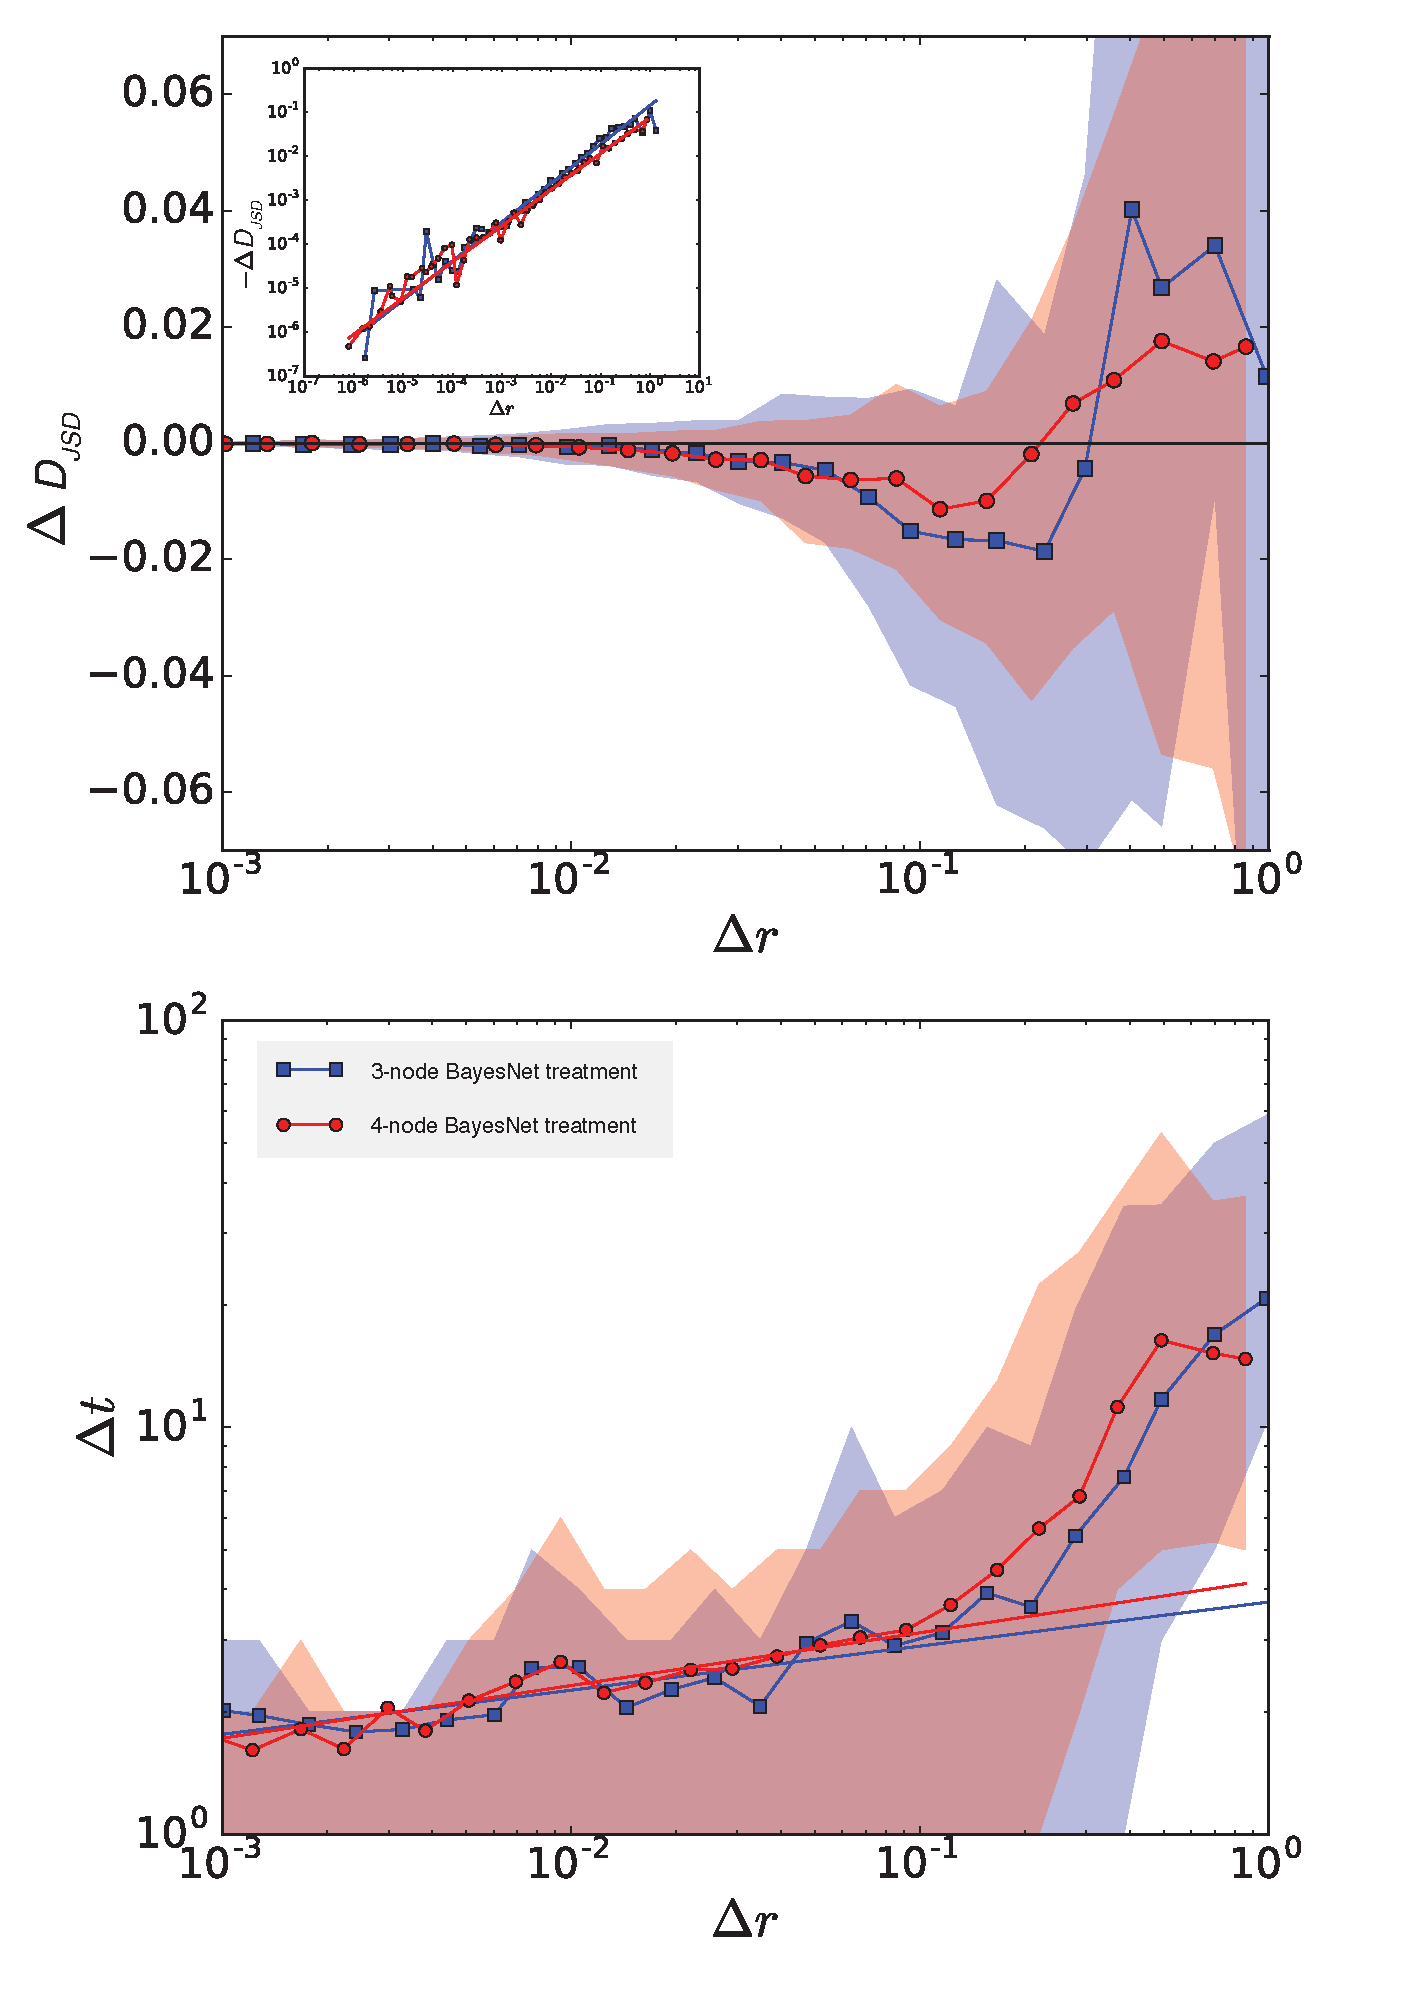
\includegraphics[width=11cm]{figures/vs_dr.eps}
\caption{{\bf A.} Evolution of the distance to the true model $D$ as a function of displacement $\Delta r$. The distance scales as $D \sim {\Delta r}^{\mu}$ with $\mu_{simple} = 0.88(1)$ [resp. $\mu_{complex} = 082(2)$]. For $\Delta r > 0.2$, $D$ becomes quickly highly uncertain, but rather positive, reflecting the {\it cost} of the making ``wild"displacements. {\bf B} For $\Delta r < 0.2$, the waiting time before a displacement decision is made scales as $\Delta t \sim \Delta r^{\gamma}$ with $\gamma_{simple} = 0.11(1)$ [resp. $\gamma_{complex} = 0.13(1)$]. For $\Delta r > 0.2$, the waiting time before a displacement decision is taken get disproportionally long (up to tens of seconds on average for displacement of 0.7 (i.e., $\approx 25\%$ of the maximum displacement distance). On both panels, blue and red areas show the 25th percentile confidence intervals.}.
%\caption{Scaling relation between $\Delta t$ and $\Delta r$ for the simple (A) and complex (B) treatments. The functions are similar for both treatments [resp. $\sim 0.44(2)$ ($p < 0.01$ , $r = 0.39$) and $\sim 0.47(2)$ ($p < 0.01$ , $r = 0.36$)]. {\bf Actually, one may see this figure differently : scaling $\Delta t \sim {\Delta r}^{0.2}$ for $\Delta r < 0.2$ and another (unknown) regime for $\Delta r > 0.2$ with waiting time getting disproportionately long $\rightarrow$ This may highlight the processing costs associated with a big jump.}}
\label{fig:vs_dr}
\end{center}
\end{figure}



